\documentclass[12pt]{exam}

\usepackage{amsmath, amssymb, amsthm, multicol}
\usepackage{graphicx}
\usepackage{textcomp}
\usepackage{tikz}

\newcommand{\vtx}[2]{node[fill,circle,inner sep=0pt, minimum size=4pt,label=#1:#2]{}}
\newcommand{\va}[1]{\vtx{above}{#1}}
\newcommand{\vb}[1]{\vtx{below}{#1}}
\newcommand{\vr}[1]{\vtx{right}{#1}}
\newcommand{\vl}[1]{\vtx{left}{#1}}
\renewcommand{\v}{\vtx{above}{}}

\def\d{\displaystyle}
\def\matrix#1{\begin{bmatrix}#1\end{bmatrix}}
\def\b{\mathbf}
\def\R{\mathbb{R}}
\def\Z{\mathbb{Z}}
\def\N{\mathbb{N}}
\def\and{\wedge}
\def\imp{\rightarrow}
\def\inv{^{-1}}
\def\st{~:~}



%\pointname{pts}
\pointsinmargin
\marginpointname{pts}
\marginbonuspointname{pts}
\addpoints
\pagestyle{head}
 \printanswers

\firstpageheader{Math 228}{\bf Quiz 9\\Solutions}{Friday, November 10}


\begin{document}

%space for name
 % \noindent {\large\bf Name:} \underline{\hspace{2.5in}}
 \vskip 1em

\begin{questions}

  \question Your friend claims she has drawn a planar graph with 6 vertices and lists the degrees of the vertices to be 5, 3, 3, 3, 2, 2.
  \begin{parts}
    \part[3] How many edges \emph{must} the graph have?  Briefly explain.  (It is not enough to draw one \emph{possible} graph; say how you know ALL graphs with these degrees have that number of edges.)
    \begin{solution}
      The number of edges is half the sum of the degrees, since each edge is counted two times when adding up the degrees.  Thus there would be $\frac{5+3+3+3+2+2}{2} = 9$ edges.
    \end{solution}
    \vfill
    \part[3]  How many faces \emph{must} the graph have?  Briefly explain.
    \begin{solution}
      If it were, the graph would satisfy Euler's formula, $v - e + f = 2$.  Thus we would have $6 - 9 + f = 2$ so $f = 5$ faces.
    \end{solution}
    \vfill

   \part[4] Could your friend's graph be isomorphic to the graph given below?  Explain.
   \[V = \{a,b,c,d,e,f\} ~~ E = \{\{a,b\}, \{a,c\}, \{a,e\}, \{a,f\}, \{b,d\}, \{b,e\}, \{c,d\}, \{c,f\}, \{d,e\}\} \]

   \begin{solution}
     No.  There is no vertex which could correspond to your friend's degree 5 vertex, since no vertex is adjacent to every other vertex.

     Here is one way we could draw the graph:

     \centerline{  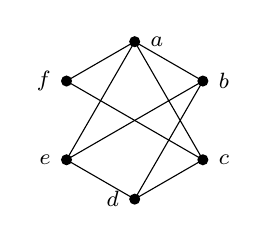
\begin{tikzpicture}
       \foreach \x in {0,...,5} {
       \coordinate (v\x) at (90-60*\x:1);}
       \draw (v3) \vl{\footnotesize \(d\)} -- (v1) \vr{\footnotesize \(b\)} -- (v4) \vl{\footnotesize \(e\)} -- (v0) \vr{\footnotesize \(a\)} -- (v2) \vr{\footnotesize \(c\)} -- (v3);
       \draw (v0) -- (v5) \vl{\footnotesize \(f\)} -- (v2) (v0) -- (v1) (v3) -- (v4);
       \end{tikzpicture}
       }
   \end{solution}
\vfill
 \end{parts}
% \question Consider the two graphs $G_1$ and $G_2$ described below:
%
%
% Graph 1: \(V = \{a,b,c,d,e\}\), \(E = \{\{a,b\}, \{a,c\}, \{a,e\}, \{b,d\}, \{b,e\}, \{c,d\}\}\).
%
%
% % Graph 2:
% % \begin{tikzpicture}[baseline=-0.5ex]
% % \foreach \x in {0,...,4} {
% % \coordinate (v\x) at (90-72*\x:.75);}
% % \draw (v3) \vl{\footnotesize \(d\)} -- (v0) \vr{\footnotesize \(a\)} -- (v2) \vr{\footnotesize \(c\)} -- (v1) \vr{\footnotesize \(b\)} -- (v4) \vl{\footnotesize \(e\)} -- (v3) -- (v2);
% % \end{tikzpicture}
%
%
%
% \begin{parts}
%   \part[2] Are the two graphs equal?  Briefly explain.
%   \begin{solution}
%     No, they are not equal.  For example, Graph 1 has an edge between $a$ and $b$ while Graph 2 does not.
%   \end{solution}
%
%   \vfill
%
%   \part[4] Are the two graphs isomorphic?  If so, give the isomorphism.  If not, explain why.
%   \begin{solution}
%     Yes they are.  We could draw Graph 1 as follows:
%
%   \centerline{  \begin{tikzpicture}
%     \foreach \x in {0,...,4} {
%     \coordinate (v\x) at (90-72*\x:.75);}
%     \draw (v3) \vl{\footnotesize \(d\)} -- (v1) \vr{\footnotesize \(b\)} -- (v4) \vl{\footnotesize \(e\)} -- (v0) \vr{\footnotesize \(a\)} -- (v2) \vr{\footnotesize \(c\)} -- (v3)  (v0) -- (v1);
%     \end{tikzpicture}
%     }
%
%     From this we can say that vertices $c$ and $d$ in $G_1$ should match up with $a$ and $b$ in $G_2$.  We need $a$ in $G_1$ to go to $e$ in $G_2$.  Then $b$ and $e$ in $G_1$ will correspond to $d$ and $e$ in $G_2$.  So one possible isomorphism is
%     \[f = \begin{pmatrix} a & b & c & d & e \\ c & d & b & e & a\end{pmatrix}\]
%   \end{solution}
%
%   \vfill
%   \vfill
%   \part[4] Give a graph with 5 vertices and 6 edges that is \underline{not} isomorphic to either of the graphs above.  Briefly explain how you know your graph is not isomorphic to the above graphs.
%
%   \begin{solution}
%     For example:
%
% \centerline{
%     \begin{tikzpicture}
% \foreach \x in {0,...,4} {
% \coordinate (v\x) at (90-72*\x:.75);}
% \draw (v3) \vl{\footnotesize \(d\)} (v0) \vr{\footnotesize \(a\)} (v2) \vr{\footnotesize \(c\)} (v1) \vr{\footnotesize \(b\)} (v4) \vl{\footnotesize \(e\)} (v0) -- (v1) (v0) -- (v2) (v0) -- (v3) (v0) -- (v4) (v1) -- (v4) (v3) -- (v2);
% \end{tikzpicture}
% }
%
% This graph has a vertex with degree 4, but neither $G_1$ nor $G_2$ do.
%   \end{solution}
%   \vfill
%   \vfill
% \end{parts}
%
% \bonusquestion[2] Bonus: Which of the graphs above are planar?
% \begin{solution}
%   All of them.  In fact, all graphs with 5 vertices and 6 edges must be planar.  Note that just because the graphs are not drawn without edges crossing does not mean that it is impossible to draw them without edges crossing.
% \end{solution}
\end{questions}
\end{document}
